\documentclass[letterpaper, 12pt, titlepage]{article}
%=======Unpackage Things===============
\usepackage{array}\usepackage{color}
\usepackage{colortbl}
\usepackage{algorithm}
\usepackage[noend]{algpseudocode}

\usepackage{graphicx}
\usepackage{amsmath}
\usepackage{amsthm}
\usepackage{listings}
%\usepackage{fullpage}
\usepackage{epsfig}
\usepackage{amsmath}
\usepackage{latexsym}
\usepackage{amssymb}
\usepackage{amstext}
\usepackage{array}
\usepackage{array}
\newcommand{\PreserveBackslash}[1]{\let\temp=\\#1\let\\=\temp}
\newcolumntype{C}[1]{>{\PreserveBackslash\centering}p{#1}}
\newcolumntype{R}[1]{>{\PreserveBackslash\raggedleft}p{#1}}
\newcolumntype{L}[1]{>{\PreserveBackslash\raggedright}p{#1}}


\begin{document}
%==title==
\title{COMP6651 Project Phase 2}
\setcounter{tocdepth}{2}
\newpage
\begin{center}
    {\huge COMP6651: Project Phase 2}


    \vspace{2cm}
    Student: Qing Gu  \hspace{5cm}
    Student ID: 6935451
   
    Student: Xuefei Shi  \hspace{5cm}
    Student ID: 6832407
\vspace{1cm}
    \vspace{1cm}

    =================================================
\end{center}

\section{Data Structure}
%Draw UML diagram here
In the program, we created two classes to store information about stations and trains. In the main program, the schedule was stored in a vector, which is initialized with the given data. During the process, the initialized data was updated to satisfy the feasibility. The figure below is the two major classes we used in program.
\begin{center}
    \small
    \centering
    \includegraphics[width=12cm]{class.ps}
    %\figcaption{UML}
    \label{uml}
\end{center}

\section{Algorithm and Time Complexity}
The algorithm I used 
%Past a screen shot of String Graph here
%Maybe I can use libpng to make it looks better


\end{document}
